%%%%%%%%%%%%%%%%%PAQUETES%%%%%%%%%%%%%%%%%%%%%%%%%%%%%%%%%%%%%%
\documentclass[a4paper,11pt]{article} %tamanho da folha, tamanho da letra, 
\usepackage{fancyhdr}%para fazer cabeçalho e rodapé
\usepackage[spanish]{babel}
\usepackage{graphicx}%para inserir imagens
\usepackage{float}%para posicionar figuras con [H]
\usepackage[left=2.5cm,top=2.5cm,right=2.5cm,bottom=4.5cm]{geometry}%margens
\usepackage[T1]{fontenc}
\usepackage{amsfonts}
\usepackage[utf8]{inputenc}
\usepackage{enumerate}
\usepackage{indentfirst}
\usepackage{lipsum}
\usepackage{biblatex}
\usepackage[hidelinks]{hyperref}

\usepackage{listings}
\usepackage{xcolor}
\definecolor{codeblue}{rgb}{0.0,0.0,0.8}
\definecolor{codegreen}{rgb}{0.0,0.6,0.0}
\definecolor{codegray}{rgb}{0.5,0.5,0.5}
\definecolor{codepurple}{rgb}{0.58,0.0,0.82}
\definecolor{codered}{rgb}{0.7,0.1,0.1}
\definecolor{backcolor}{rgb}{0.95,0.95,0.92}

\lstdefinestyle{javascript}{
   language=JavaScript,
   backgroundcolor=\color{backcolor},
   basicstyle=\ttfamily\small,
   keywordstyle=\color{codeblue}\bfseries,
   stringstyle=\color{codegreen},
   commentstyle=\color{codegray}\itshape,
   numbers=left,
   numberstyle=\tiny\color{codegray},
   frame=single,
   breaklines=true,
   showstringspaces=false,
   breakatwhitespace=false,
   captionpos=b,
   keepspaces=true
}

% Definición del lenguaje JavaScript antes de crear el estilo
\lstdefinelanguage{JavaScript}{
   keywords={break, case, catch, class, const, continue, debugger, default, delete, do, else, export, extends, finally, for, function, if, import, in, instanceof, new, return, super, switch, this, throw, try, typeof, var, void, while, with, yield, let, async, await},
   keywordstyle=\color{codeblue}\bfseries,
   ndkeywords={boolean, number, string, undefined, null, NaN, console, true, false},
   ndkeywordstyle=\color{codepurple}\bfseries,
   identifierstyle=\color{black},
   sensitive=true,
   comment=[l]{//},
   morecomment=[s]{/*}{*/},
   commentstyle=\color{codegray}\itshape,
   stringstyle=\color{codegreen},
   morestring=[b]',
   morestring=[b]",
   morestring=[b]`
}

\addbibresource{books.bib}
%--------------------------------
%%%%%%%%%%%%%%%%%%%ENCABEZADO%%%%%%%%%%%%%%%%%%%%%%%%%%%%%%%%%%%%
\pagestyle{fancy}
\renewcommand{\headrulewidth}{0pt} %altera a espessura da linha do cabeçalho, se colocarmos 0pt não aparecerá a linha.
\fancyhead[R]{
\includegraphics[height=45pt]{logo.jpeg}
}%figura ao lado direito do cabeçalho
\lhead{ \textbf{Universidad Nacional de Loja} \\ \textbf{Carrera en Computación} \\ \textbf{Facultad de Energía las Industrias y los Recursos Naturales no Renovables}}%texto ao lado esquerdo do cabeçalho
\setlength{\headheight}{80pt}%tamanho do ambiente do cabeçalho
%%%%%%%%%%%%%%%%%%%%RODAPÉ%%%%%%%%%%%%%%%%%%%%%%%%%%%%%%%%%%%%%%%%%%%%%
\cfoot{}%centro do rodapé vazio
\rfoot{\thepage} %numeração das páginas ao lado direto do rodapé

%%%%%%%%%%%%%%%%%%%%%%%%%DATOS%%%%%%%%%%%%%%%%%%%%%%%%%%%%%
\begin{document}
%%%%%%%%%%%%%%%%%%%%%%%%%PORTADA%%%%%%%%%%%%%%%%%%%%%%%%%%%%%
\begin{titlepage}
`   \centering
   {\large \textbf{UNIVERSIDAD NACIONAL DE LOJA}\par}
   \vspace{0.4cm}
   {\large \textbf{CARRERA DE COMPUTACIÓN}\par}
   \vspace{2cm}
   {\large Asignatura: \textbf{Estructura de Datos}\par}
   \vspace{2cm}
   {\Large \textbf{Informe Técnico}\par}
   \vspace{0.3cm}
   {\large Avance 4 del Proyecto ABP (Unidad 01)\par}
   \vspace{0.3cm}
   {\large Implementación de Navegación Bidireccional (ListaDoble),\\
   Pruebas Unitarias de Integración y Protocolo de Entrega EVA\par}
   \vspace{2cm}
   {\large \textbf{Grupo N.° 03}\par}
   \vspace{1cm}
   {\large \textbf{Integrantes:}\par}
   \vspace{0.3cm}
   \begin{tabular}{l}
      Domenica Narváez \\
      Dario Chillogallo \\
      Galo Benitez \\
      Yandry Campoverde \\
      Jose Maldonado \\
   \end{tabular}'

   % ---------- REPOSITORIO ----------
   \vspace{1cm}
   {\large \textbf{Repositorio en GitHub:}\par}
   \vspace{0.3cm}
   {\large \url{https://github.com/usuario/nombre-repositorio}\par}

   \vfill
   {\large Loja, \today\par}
\end{titlepage}

%%%%%%%%%%%%%%%%%%%%%%%%%TEXTO%%%%%%%%%%%%%%%%%%%%%%%%%%%%%

\section*{Actividad}
Resolución de ejercicios conceptuales mediante la representación gráfica de bloques de memoria (Stack y Heap), direcciones simbólicas y evolución de referencias ante operaciones de instanciación y liberación.Trabajo autónomo colaborativo orientado al diseño de baterías de pruebas unitarias y a la integración del módulo de listas en el repositorio de control de versiones del equipo.

\section*{Desarrollo}

\subsection{Caso de Estudio 1: Shared Lexical Context Leak}
\begin{lstlisting}[language=JavaScript,style=javascript]
let ejecutorGlobal = null;

function crearProcesadorResiduos() {
   //Asignacion de 10 MB en el Heap
   let datosMasivos = new Array(10 * 1024 * 1024).fill("DATA_CRITICA");
   let copiaAnterior = ejecutorGlobal;

   //Funcion interna 1: NUNCA se invoca directamente, pero utiliza datosMasivos
   let funcionRetenida = function () {
      if (datosMasivos) {
      console.log("Referencia activa a datos masivos");
      }
   };

   //Funcion interna 2: Sobrevive asignandose a la variable global
   ejecutorGlobal = function () {
      console.log("Ejecutando proceso liviano...");
      if (copiaAnterior) {
      copiaAnterior();
      }
   };

// Simulacion de llamadas repetidas
setInterval(() => {
   crearProcesadorResiduos();
   console.log(`Heap usado: ${(process.memoryUsage().heapUsed / 1024 / 1024).toFixed(2)} MB`);
}, 1000);
}
\end{lstlisting}
\begin{itemize}
   \item \textbf{Primera ejecucion}
\end{itemize}
\begin{figure}[H]
\centering
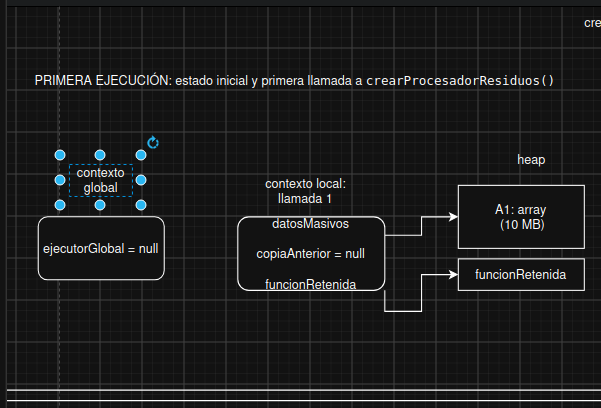
\includegraphics[width=0.6\linewidth]{figuras/01ejercicio/imagen1.1.png}
\caption{Primera ejecución: estado inicial y primera llamada a \texttt{crearProcesadorResiduos()}.}
\end{figure}
Al llamar por primera vez a \texttt{crearProcesadorResiduos()} se crea su contexto local. En el Heap se reservan el arreglo \texttt{datosMasivos} (A1, 10 MB) y \texttt{funcionRetenida}. Como \texttt{ejecutorGlobal} todavía es \texttt{null}, \texttt{copiaAnterior} también vale \texttt{null}.

\begin{figure}[H]
\centering
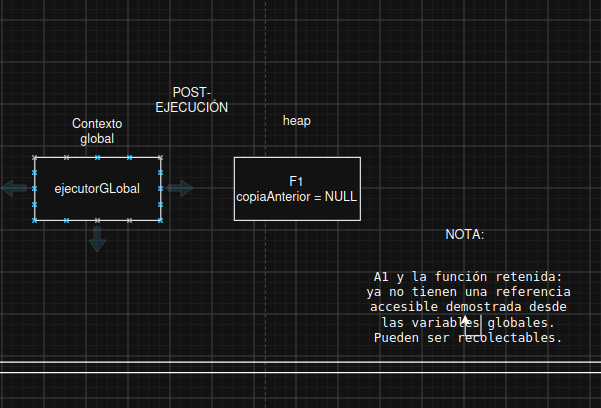
\includegraphics[width=0.6\linewidth]{figuras/01ejercicio/imagen1.2.png}
\caption{Primera ejecución: estado post-ejecución.}
\end{figure}
Al terminar la llamada, el contexto local desaparece del Stack y \texttt{ejecutorGlobal} queda apuntando a la función F1, cuyo \texttt{copiaAnterior} es \texttt{null}. Las funciones internas comparten el mismo contexto léxico, que contiene a \texttt{datosMasivos}; por eso A1 puede seguir ocupando memoria aunque F1 no lo use.

\begin{itemize}
   \item \textbf{Segunda ejecucion}
\end{itemize}
\begin{figure}[H]
\centering
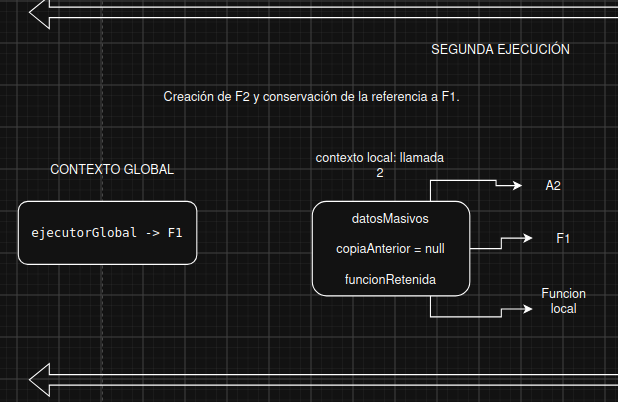
\includegraphics[width=0.6\linewidth]{figuras/01ejercicio/imagen2.1.png}
\caption{Segunda ejecución: creación de F2 y conservación de la referencia a F1.}
\end{figure}
En la segunda llamada se crea un nuevo contexto local con un nuevo arreglo (A2, 10 MB) y una nueva función. Esta vez \texttt{copiaAnterior} guarda la referencia a F1, que era el valor de \texttt{ejecutorGlobal}.

\begin{figure}[H]
\centering
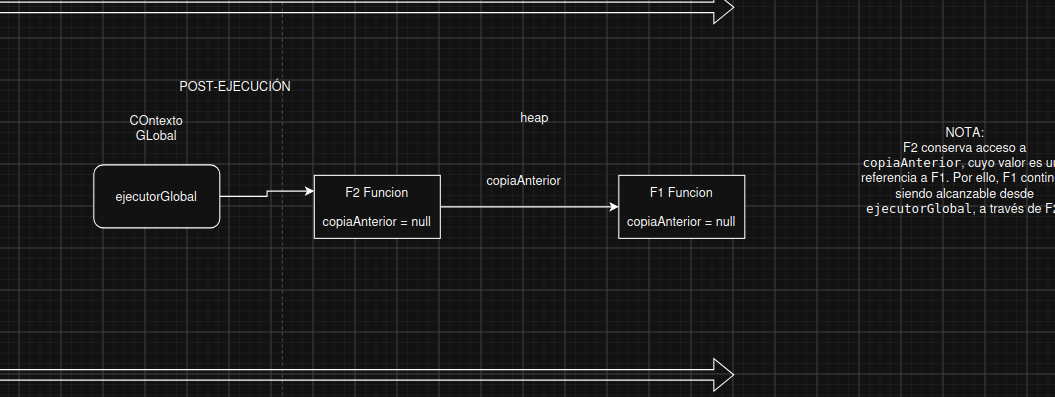
\includegraphics[width=0.85\linewidth]{figuras/01ejercicio/imagen2.2.png}
\caption{Segunda ejecución: estado post-ejecución.}
\end{figure}
Al finalizar, \texttt{ejecutorGlobal} apunta a F2, y F2 conserva en \texttt{copiaAnterior} la referencia a F1. F1 sigue siendo alcanzable desde la variable global a través de F2, por lo que no puede ser liberada.

\begin{itemize}
   \item \textbf{Tercera ejecucion}
\end{itemize}
\begin{figure}[H]
\centering
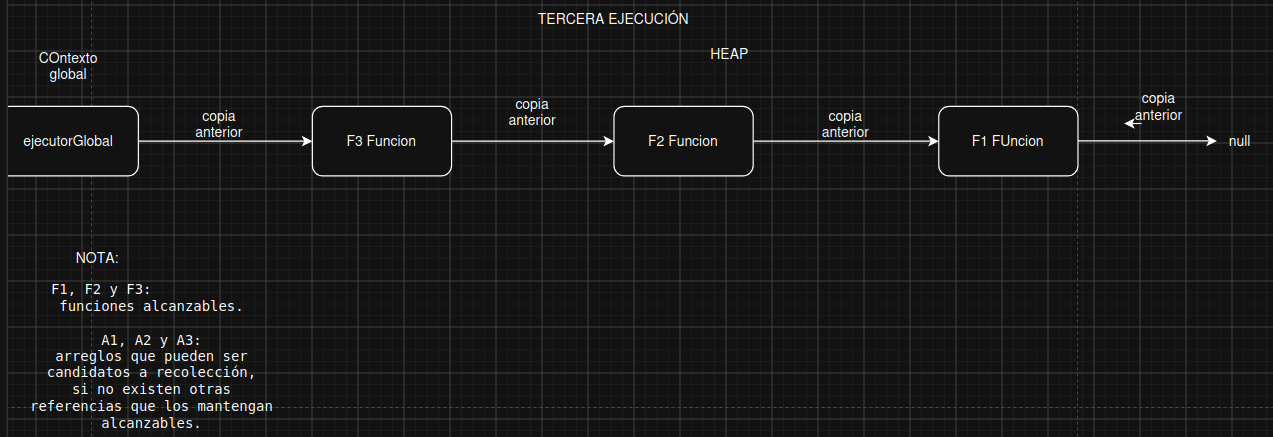
\includegraphics[width=0.95\linewidth]{figuras/01ejercicio/imagen3.png}
\caption{Tercera ejecución: cadena de funciones alcanzables desde \texttt{ejecutorGlobal}.}
\end{figure}
Con la tercera llamada se forma una cadena \texttt{ejecutorGlobal} $\rightarrow$ F3 $\rightarrow$ F2 $\rightarrow$ F1 $\rightarrow$ \texttt{null}. Cada nueva ejecución añade un eslabón y el uso de memoria crece de forma continua, que es el patrón de una fuga de memoria.


\subsection{Caso de Estudio 2: Grafo Circular y Referencias Débiles}
\begin{lstlisting}[language=Javascript, style=javascript]
// Caso de Estudio 2: Grafo Circular y Referencias Debiles
class NodoGrafo {
   constructor(id) {
      this.id = id;
      this.vecinos = [];
   }

   conectarCon(nodo) {
      this.vecinos.push(nodo);
   }
}

function construirGrafoCiclico() {
   let nodoA = new NodoGrafo("A");
   let nodoB = new NodoGrafo("B");
   let nodoC = new NodoGrafo("C");

   // Conexion circular bidireccional
   nodoA.conectarCon(nodoB);
   nodoB.conectarCon(nodoC);
   nodoC.conectarCon(nodoA);

   // Registro en un gestor centralizado
   gestorCache.set(nodoA.id, nodoA);

   return nodoA.id;
}

const gestorCache = new Map(); // Map o WeakMap

let idRaiz = construirGrafoCiclico();

// El estudiante debe analizar que sucede al ejecutar:
// gestorCache.delete(idRaiz);
\end{lstlisting}
\begin{itemize}
   \item \textbf{Estado A:} dentro de \texttt{construirGrafoCiclico}
\end{itemize}
\begin{figure}[H]
\centering
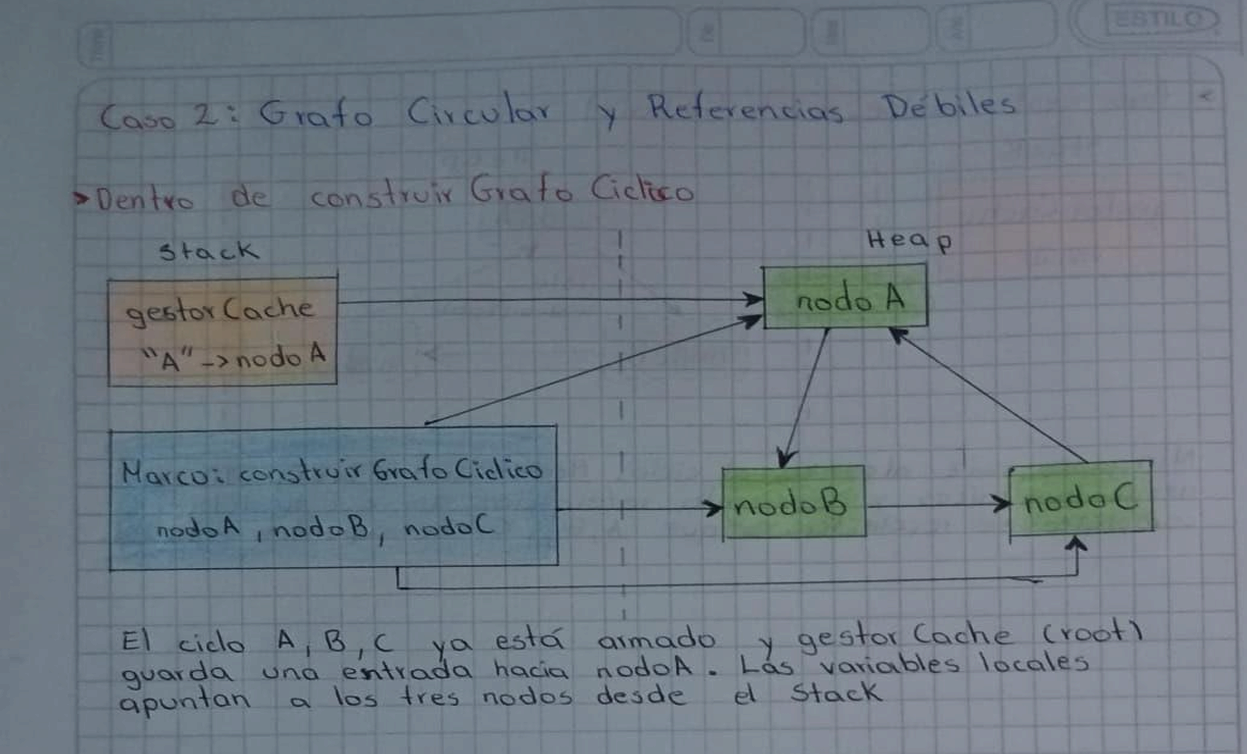
\includegraphics[width=0.8\linewidth]{figuras/02ejercicio/esatdoA.png}
\caption{Estado A: dentro de \texttt{construirGrafoCiclico}.}
\end{figure}
Se crean los tres nodos y se conectan en círculo: A apunta a B, B a C y C a A. Las variables locales del marco de la función apuntan a los tres nodos en el Heap, y además \texttt{gestorCache} guarda la entrada \texttt{"A"} $\rightarrow$ \texttt{nodoA}. En este momento todo está vivo.

\begin{itemize}
   \item \textbf{Estado B:} tras retornar la función
\end{itemize}
\begin{figure}[H]
\centering
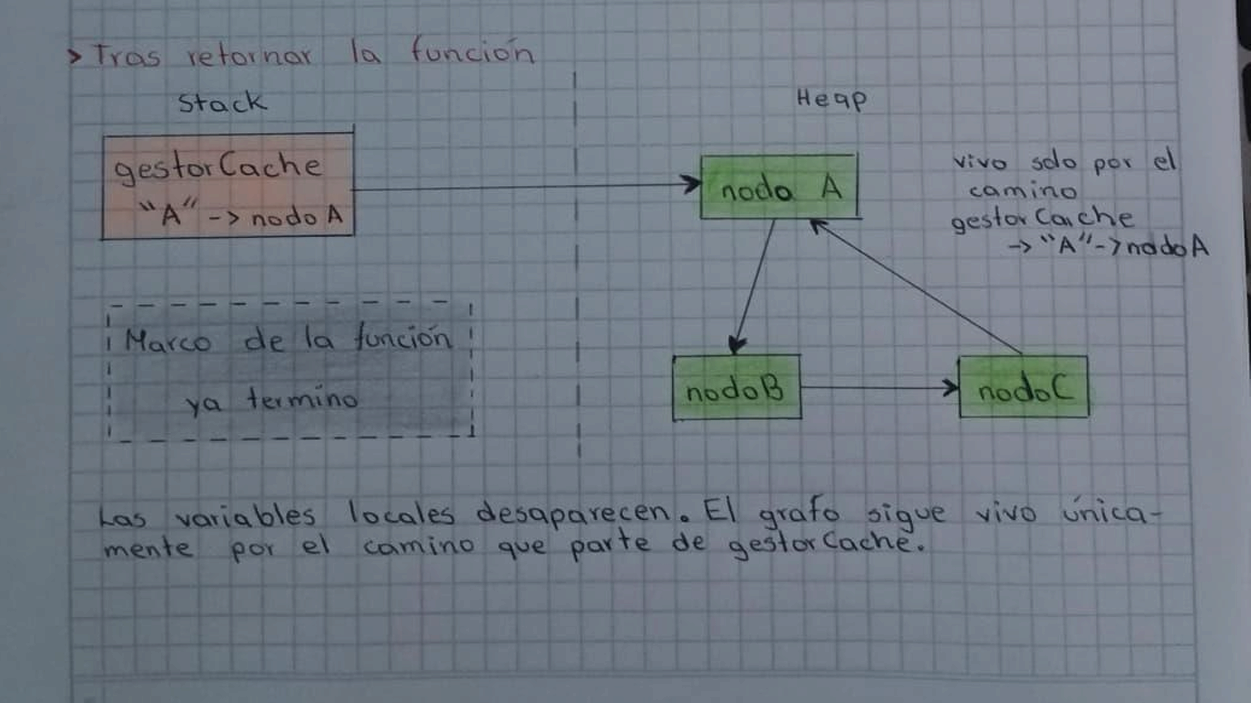
\includegraphics[width=0.8\linewidth]{figuras/02ejercicio/estadoB.png}
\caption{Estado B: tras retornar la función.}
\end{figure}
La función termina y su marco desaparece del Stack junto con \texttt{nodoA}, \texttt{nodoB} y \texttt{nodoC}. Los nodos siguen vivos solo por el camino \texttt{gestorCache} $\rightarrow$ \texttt{"A"} $\rightarrow$ \texttt{nodoA}, desde donde se llega a B y C por las flechas del ciclo.

\begin{itemize}
   \item \textbf{Estado C:} tras \texttt{gestorCache.delete(idRaiz)}
\end{itemize}
\begin{figure}[H]
\centering
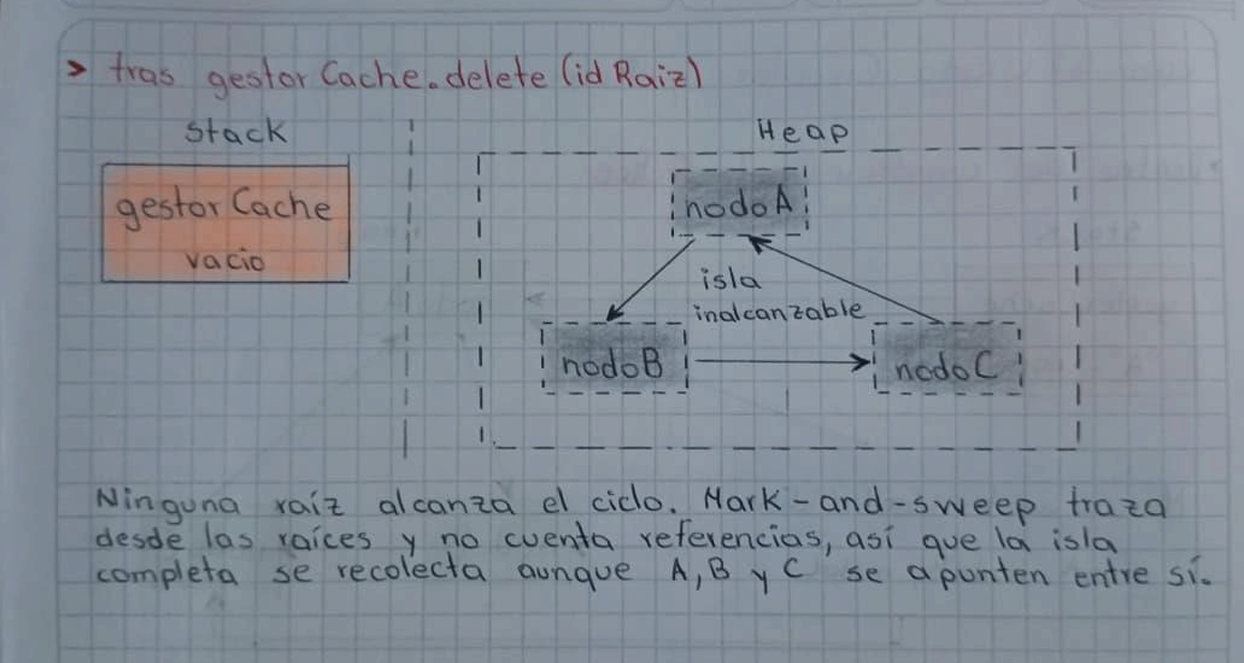
\includegraphics[width=0.8\linewidth]{figuras/02ejercicio/estadoC.png}
\caption{Estado C: tras \texttt{gestorCache.delete(idRaiz)}.}
\end{figure}
Al borrar la entrada del Map ninguna raíz llega al grafo, y los tres nodos quedan como una isla inalcanzable aunque se sigan apuntando entre sí. El recolector usa \textit{mark-and-sweep}: parte de las raíces, marca lo que alcanza y libera el resto, así que el ciclo se recolecta completo.


\subsection{Caso de Estudio 3: Event Loop Queue \& Retención por Callbacks}
\begin{lstlisting}[language=Javascript, style=javascript]
const EventEmitter = require('events');
const emisorGlobal = new EventEmitter();

class GestorSesionUsuario {
    constructor(idUsuario) {
        this.idUsuario = idUsuario;
        // Reserva de 5 MB de datos por sesion
        this.bufferSesion = new Uint8Array(5 * 1024 * 1024);
        
        // Suscripcion al emisor global
        this.oyenteEvento = () => {
            this.actualizarActividad();
        };
        
        emisorGlobal.on('pingSistema', this.oyenteEvento);
    }

    actualizarActividad() {
        console.log("Sesion ${this.idUsuario} activa.");
    }

    cerrarSesion() {
        console.log(`Cerrando sesion de ${this.idUsuario}`);
        // NOTA: El desarrollador olvido desregistrar el evento en emisorGlobal
    }
    }

    function simularTrafico() {
    for (let i = 0; i < 50; i++) {
        let usuario = new GestorSesionUsuario(`USR_${i}`);
        usuario.cerrarSesion();
        // La variable local `usuario` sale de alcance (Stack) al terminar la iteracion
    }
}

simularTrafico();
// Forzar la ejecucion del evento global
emisorGlobal.emit('pingSistema');
\end{lstlisting}
\begin{itemize}
   \item \textbf{Ejecucion 1:} creación de la primera sesión
\end{itemize}
\begin{figure}[H]
\centering
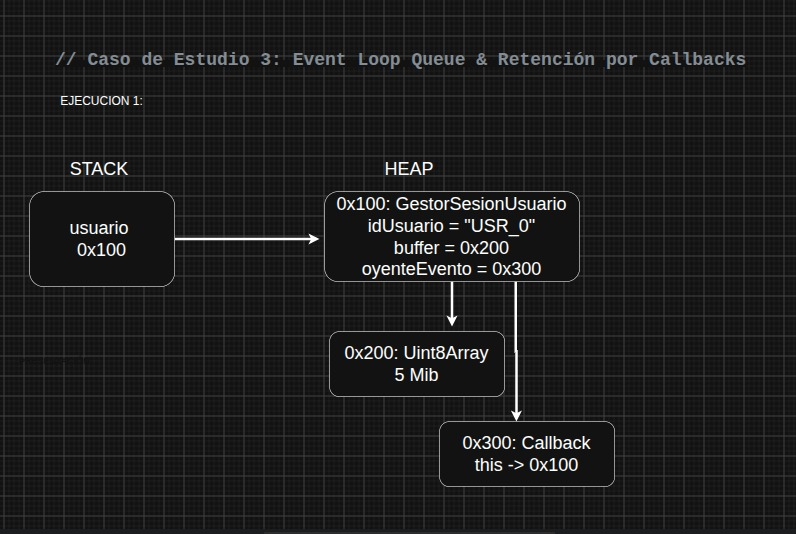
\includegraphics[width=0.6\linewidth]{figuras/03ejercicio/EJECUCION1.jpeg}
\caption{Ejecución 1: primera sesión (\texttt{USR\_0}) en Stack y Heap.}
\end{figure}
Al crear el primer usuario (\texttt{USR\_0}) se instancia un \texttt{GestorSesionUsuario} en el Heap (0x100), al que apunta la variable local \texttt{usuario}. El objeto contiene un buffer de 5 MiB (0x200) y un callback (0x300) que conserva una referencia al objeto mediante \texttt{this} y se registra en \texttt{emisorGlobal}.

\begin{itemize}
   \item \textbf{Ejecucion 2:} 50 sesiones creadas
\end{itemize}
\begin{figure}[H]
\centering
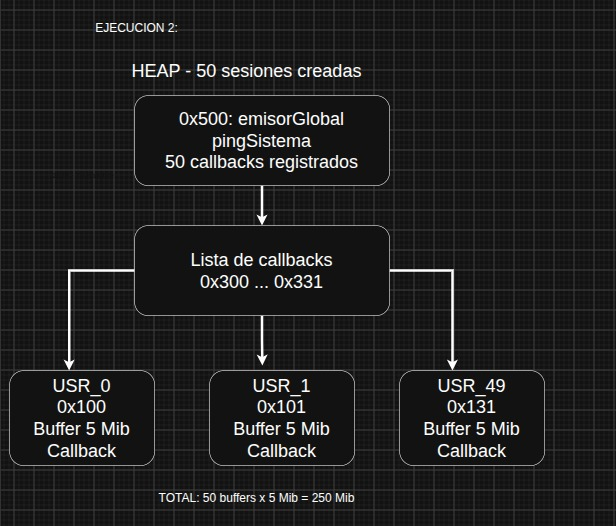
\includegraphics[width=0.5\linewidth]{figuras/03ejercicio/EJECUCION2.jpeg}
\caption{Ejecución 2: 50 sesiones creadas y registradas en \texttt{emisorGlobal}.}
\end{figure}
Durante \texttt{simularTrafico()} se crean 50 sesiones, cada una con su buffer de 5 MiB y su callback registrado en el evento \texttt{pingSistema}. En total hay 50 buffers $\times$ 5 MiB = 250 MiB en el Heap.

\begin{itemize}
   \item \textbf{Ejecucion 3:} fin de \texttt{simularTrafico()}
\end{itemize}
\begin{figure}[H]
\centering
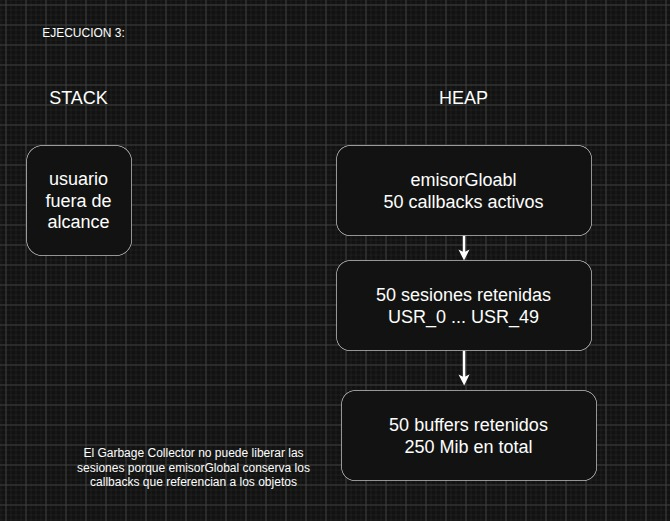
\includegraphics[width=0.5\linewidth]{figuras/03ejercicio/EJECUCION3.jpeg}
\caption{Ejecución 3: sesiones retenidas tras salir de alcance la variable \texttt{usuario}.}
\end{figure}
Al terminar el ciclo la variable \texttt{usuario} sale de alcance, pero \texttt{cerrarSesion()} solo escribe un mensaje y no desregistra el evento. \texttt{emisorGlobal} conserva los 50 callbacks, que referencian a sus objetos, por lo que el Garbage Collector no puede liberar las sesiones ni sus 250 MiB.

\begin{itemize}
   \item \textbf{Ejecucion 4:} emisión de \texttt{pingSistema}
\end{itemize}
\begin{figure}[H]
\centering
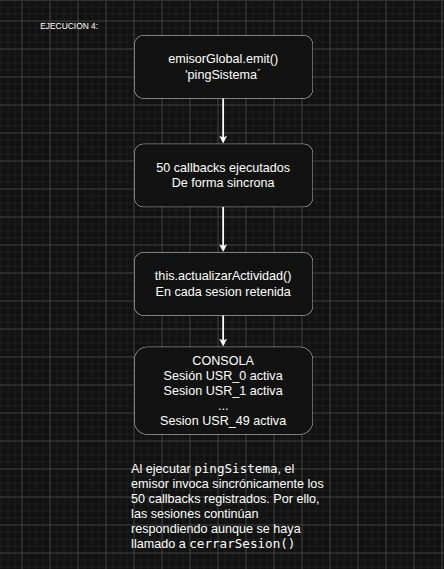
\includegraphics[width=0.4\linewidth]{figuras/03ejercicio/EJECUCION4.jpeg}
\caption{Ejecución 4: \texttt{emisorGlobal.emit('pingSistema')}.}
\end{figure}
Al ejecutar \texttt{emisorGlobal.emit('pingSistema')} se invocan de forma síncrona los 50 callbacks, y cada uno llama a \texttt{actualizarActividad()} sobre su sesión. Esto demuestra que las sesiones ``cerradas'' siguen en memoria y respondiendo al evento.

\section*{Conclusiones}

\begin{itemize}
   \item C01: En el Caso 1, las funciones internas comparten un mismo contexto léxico, por lo que una función global puede retener datos pesados que no usa. Al encadenarse mediante \texttt{copiaAnterior}, cada llamada añade 10 MB que no se liberan, lo que produce una fuga de memoria progresiva.
   \item C02: En el Caso 2, el recolector de basura (\textit{mark-and-sweep}) decide qué liberar según la alcanzabilidad desde las raíces y no según el número de referencias. Por eso un grafo circular se recolecta completo cuando deja de ser alcanzable, aunque sus nodos se apunten entre sí.
   \item C03: En el Caso 3, un callback registrado en un emisor global mantiene vivo al objeto que lo creó mediante \texttt{this}. Mientras no se desregistre el oyente, las 50 sesiones y sus 250 MiB siguen alcanzables aunque se llame a \texttt{cerrarSesion()}.
   \item C04: En conjunto, los tres casos muestran que las fugas de memoria en JavaScript suelen deberse a referencias olvidadas desde raíces globales (variables, mapas o emisores de eventos). Liberar recursos de forma explícita, como desregistrar eventos con \texttt{removeListener} o eliminar entradas de cachés, y diagramar el Stack y el Heap permite detectar estos problemas.
\end{itemize}


\end{document}